\documentclass[12pt,fleqn]{article}\usepackage{../common}
\begin{document}
En Yakin k-Komsu (k-Nearest Neighbor)

Yapay Ogrenim alaninda ornek bazli ogrenen algoritmalardan bilinen kNN,
egitim verinin kendisini siniflama (classification) amacli olarak kullanir,
yeni bir model ortaya cikartmaz. Algoritma soyle isler: etiketleri bilinen
egitim verisi alinir ve bir kenarda tutulur. Yeni bir veri noktasi
gorulunce bu veriye geri donulur ve o noktaya ``en yakin'' k tane nokta
bulunur. Daha sonra bu noktalarin etiketlerine bakilir ve cogunlugun
etiketi ne ise, o etiket yeni noktanin etiketi olarak kabul edilir.

``En yakin'' sozu bir kordinat sistemi anlamina geliyor, ve kNN, aynen
k-Means ve diger pek cok kordinatsal ogrenme yontemi gibi eldeki cok
boyutlu veri noktalarinin elemanlarini bir kordinat sistemindeymis gibi
gorur. Kiyasla mesela APriori gibi bir algoritma metin bazli veriyle oldugu
gibi calisabilirdi.

Peki arama baglaminda, bir veri obegi icinden en yakin noktalari bulmanin
en basit yolu nedir? Listeyi bastan sonra taramak (kaba kuvvet yontemi
-brute force-) ve her listedeki nokta ile yeni nokta arasindaki mesafeyi
teker teker hesaplayip en yakin k taneyi icinden secmek bir yontem. Bu
basit algoritmanin yuku $O(N)$'dir. Eger tek bir nokta ariyor olsaydik,
bu kabul edilebilir olabilirdi. Fakat genellikle bir siniflayici
algoritmanin surekli islemesi, mesela bir online site icin gunde
milyonlarca kez bazi kararlari almasi gerekebilir. Bu durumda ve $N$'in cok
buyuk oldugu sartlarda, ustteki hiz bile yeterli olmayabilir.

Arama islemini daha hizli yapmanin yollari var. Akilli arama algoritmalari
kullanarak egitim verilerini bir agac yapisi uzerinden tarayip erisim
hizini $O(\log N)$'e indirmek mumkundur.

K�re Aga�lar� (Ball Tree, BT) 

Bir noktanin diger noktalara yakin olup olmadiginin hesabinda yapilmasi
gereken en pahali islem nedir? Mesafe hesabidir. BT algoritmasinin puf
noktasi bu hesabi yapmadan, noktalara degil, noktalari kapsayan
``kurelere'' bakarak hiz kazandirmasidir. Noktalarin her biri yerine o
noktalari temsil eden kurenin mihenk noktasina (pivot -bu nokta kure
icindeki noktalarin ortalamasal olarak merkezi de olabilir, herhangi bir
baska nokta da-) bakilir, ve oraya olan mesafeye gore bir kure altindaki
noktalara olabilecek en az ve en fazla uzaklik hemen anlasilmis olur.

Mesela elimizde alttaki gibi noktalar var ve kureyi olusturduk. 

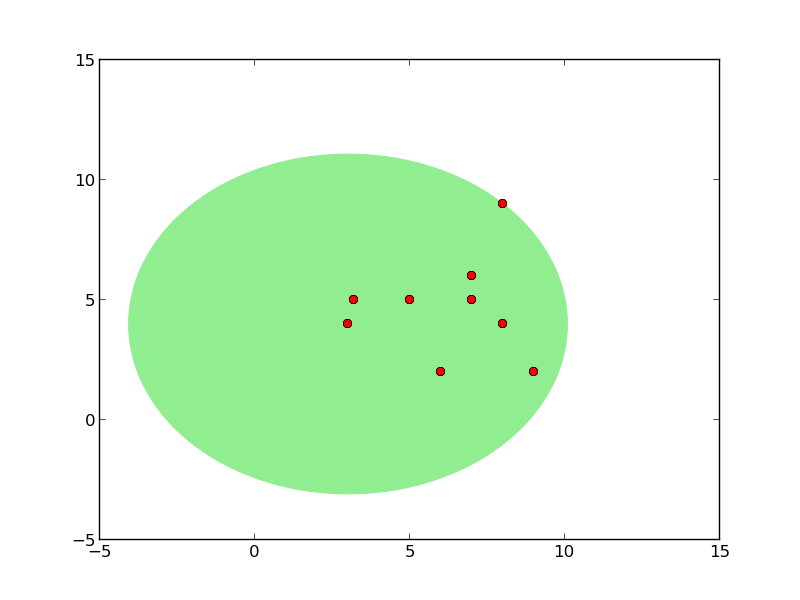
\includegraphics[height=6cm]{pics/knn0.png}

Bu kureyi kullanarak kure disindaki herhangi bir nokta $q$'nun kuredeki
``diger tum noktalar $x$'e'' olabilecegi en az mesafenin ne olacagini
ucgensel esitsizlik ile anlayabiliriz.

Ucgensel esitsizlik 

\[ |x-y| \le |x-z| + |z-y| \]

$||$ operatoru norm operatoru anlamina gelir ve uzaklik hesabinin
genellestirilmis halidir. Konu hakkinda daha fazla detay icin {\em
  Fonksinel Analiz} ders notlarimiza bakabilirsiniz. Kisaca soylenmek
istenen iki nokta arasinda direk gitmek yerine yolu uzatirsak, mesafe
artacagidir. Tabii uzaklik, yol, nokta gibi kavramlar tamamen soyut matematiksel
ortamda da isleyecek sekilde ayarlanmistir. Mesela mesafe (norm) kavramini
degistirebiliriz, Oklitsel yerine Manhattan mesafesi kullaniriz, fakat bu
kavram bir norm oldugu ve belirttigimiz uzayda gecerli oldugu icin ucgensel
esitsizlik uzerine kurulmus tum diger kurallar gecerli olur. 

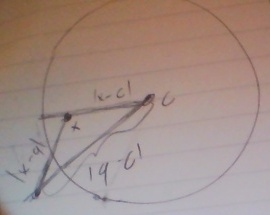
\includegraphics[height=5cm]{pics/tri1.png}

Simdi diyelim ki disaridaki bir $q$ noktasindan bir kure icindeki diger tum
$x$ noktalarina olan mesafe hakkinda bir seyler soylemek istiyoruz. Ustteki
sekilden bir ucgensel esitsizlik cikartabiliriz,

\[ |x-c| + |x-q| \ge |q-c|  \]

Bunun dogru bir ifade oldugunu biliyoruz. Peki simdi yaricapi bu ise dahil
edelim, cunku yaricap hesabi bir kere yapilip kure seviyesinde depolanacak
ve bir daha hesaplanmasi gerekmeyecek, yani algoritmayi hizlandiracak bir
sey olabilir bu, o zaman eger $|x-c|$ yerine yaricapi kullanirsak,
esitsizlik hala gecerli olur, sol taraf zaten buyuktu, simdi daha da buyuk
olacak, 

\[ radius + |x-q| \ge |q-c|  \]

Bunu nasil boyle kesin bilebiliyoruz? Cunku BT algoritmasi radius'u
$|x-c|$'ten kesinlikle daha buyuk olacak sekilde secer). Simdi yaricapi
saga gecirelim,

\[ |x-q| \ge |q-c| - radius \]

Boylece guzel bir tanim elde ettik. Yeni noktanin kuredeki herhangi bir
nokta $x$'e olan uzakligi, yeni noktanin mihenke olan uzakliginin yaricapi
cikartilmis halinden {\em muhakkak} fazladir. Yani bu cikartma isleminden
ele gecen rakam yeni noktanin $x$'e uzakligina bir ``alt sinir (lower
bound)'' olarak kabul edilebilir. Diger tum mesafeler bu rakamdan daha
buyuk olacaktir. Ne elde ettik? Sadece bir yeni nokta, mihenk ve yaricap
kullanarak kuredeki ``diger tum noktalar hakkinda'' bir irdeleme yapmamiz
mumkun olacak. Bu noktalara teker teker bakmamiz gerekmeyecek. Bunun nasil
ise yaradigini algoritma detaylarinda gorecegiz.

Benzer sekilde 

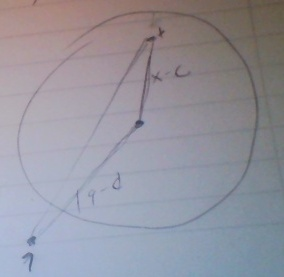
\includegraphics[height=5cm]{pics/tri2.png}

Bu ne diyor? 

\[ |q-c| + |x-c| \ge |q-x| \]

$|x-c|$ yerine yaricap kullanirsak, sol taraf buyuyecegi icin buyukluk hala
buyukluk olarak kalir, 

\[ |q-c| + radius \ge |q-x| \]

Ve yine daha genel ve hizli hesaplanan bir kural elde ettik (onceki
ifadeye benzemesi icin yer duzenlemesi yapalim)

\[ |q-x| \le |q-c| + radius \]

Bu ifade ne diyor? Yeni noktanin mihenke olan uzakligina yaricap
``eklenirse'' bu uzakliktan, buyuklukten daha buyuk bir yeni nokta / kure
 mesafesi olamaz, kuredeki hangi nokta olursa olsun. Bu esitsizlik te bize
 bir ust sinir (upper bound) vermis oldu. 

Algoritma

Kure Agaclari (BT) metotu once kureleri, agaclari olusturmalidir. Bu
kureler hiyerarsik sekilde planlanir, tum noktalarin icinde oldugu bir ``en
ust kure'' vardir her kurenin iki tane cocuk kuresi olabilir. Belli bir
(disaridan tanimlanan) minimum $r_{min}$ veri noktasina gelinceye kadar
sadece noktalari geometrik olarak kapsamakla goreli kureler olusturulur,
kureler noktalari sahiplenmezler. Fakat bu $r_{min}$ sayisina erisince
(artik oldukca alttaki) kurelerin uzerine noktalar konacaktir.

Once tek kurenin olusturulusuna bakalim. Bir kure olusumu icin eldeki veri
icinden herhangi bir tanesi mihenk olarak kabul edilebilir. Daha sonra bu
mihenkten diger tum noktalara olan uzaklik olculur, ve en fazla, en buyuk
olan uzaklik yaricap olarak kabul edilir (her seyi kapsayabilmesi icin).

Not: Bu arada ``tum diger noktalara bakilmasi'' dedik, bundan kacinmaya
calismiyor muyduk?  Fakat dikkat, ``kure olusturulmasi'' evresindeyiz, k
tane yakin nokta arama evresinde degiliz. Yapmaya calistigimiz aramalari
hizlandirmak - egitim / kure olusturmasi bir kez yapilacak ve bu egitilmis
kureler bir kenarda tutulacak ve surekli aramalar icin ardi ardina
kullanilacaklar.

Kureyi olusturmanin algoritmasi soyledir: verilen noktalar icinde herhangi
birisi mihenk olarak secilir. Sonra bu noktadan en uzakta olan nokta $f_1$,
sonra $f_1$'den en uzakta olan nokta $f_2$ secilir. Sonra tum noktalara
teker teker bakilir ve $f_1$'e yakin olanlar bir gruba, $f_2$'ye yakin
olanlar bir gruba ayrilir. 

\lstinputlisting[language=Python]{knn.py}

\lstinputlisting[language=Python]{dist.py}

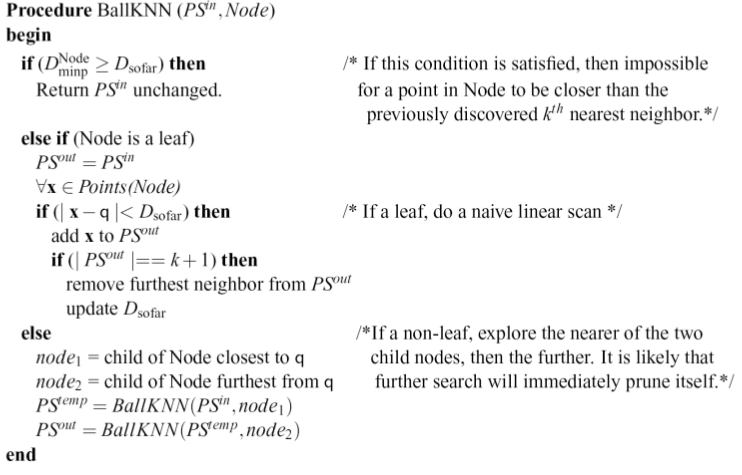
\includegraphics[height=7cm]{alg.png}

Bu iki grup, o anda islemekte oldugumuz agac dugumun (node) iki cocuklari
olacaktir. Cocuk noktalari kararlastirildiktan sonra artik sonraki asamaya
gecilir, fonksiyon \verb!form_tree! bu cocuk noktalari alarak, ayri ayri,
her cocuk grubu icin ozyineli (recursive) olarak kendi kendini
cagirir. Kendi kendini cagiran \verb!form_tree!, tekrar basladiginda
kendini yeni (bir) nokta grubu ve yeni bir dugum objesi ile basbasa bulur,
ve hicbir seyden habersiz olarak isleme koyulur. Tabii her ozyineli cagri
yeni dugum objesini yaratirken bir referansi ustteki ebeveyn dugume koymayi
unutmamistir, boylece ozyineli fonksiyon dunyadan habersiz olsa bile,
agacin en ustunden en altina kesintisiz bir baglanti zinciri hep elimizde
olur.

Not: \verb!form_tree! icinde bir numara yaptik, tum noktalarin $f_1$'e olan
uzakligi \verb!dist1!, $f_2$'e olan uzakligi ise \verb!dist2!. Sonra
\verb!diffs = dist1-dist2! ile bu iki uzakligi birbirinden cikartiyoruz ve
mesela \verb!points[diffs <= 0]! ile $f_1$'e yakin olanlari buluyoruz,
cunku bir tarafta $f_1$'e yakinlik 4 diger tarafta $f_2$'ye yakinlik 6 ise,
4-6=-2 ie o nokta $f_1$'e yakin demektir. Ufak bir numara ile Numpy
dilimleme (slicing) teknigini kullanabilmis olduk ve bu onemli cunku
boylece \verb!for! dongusu yazmiyoruz, Numpy'in arka planda C ile yazilmis
hizli rutinlerini kullaniyoruz.

Ek bazi bilgiler: kurelerin sinirlari kesisebilir. 

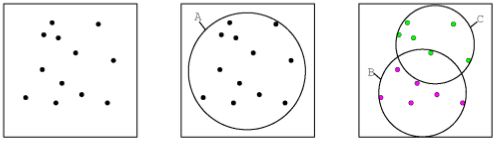
\includegraphics[height=3cm]{pics/balls1.png}

Arama 

Ustteki imaj icinde $BallKNN$ olarak gosterilen ve bizim kodda
\verb!search_tree! olarak anilan fonksiyon arama fonksiyonu. Aranan
\verb!new_point!'e olan k en yakin diger veri noktalar. Disaridan verilen
degisken \verb!knn_matches! uzerinde fonksiyon ozyineli bir sekilde arama
yaparken ``o ana kadar bulunmus en yakin k nokta'' ve o noktalarin
\verb!new_point!'e olan en yakin mesafesi saklanir, arama isleyisi
sirasinda \verb!knn_matches!, \verb!knn_matches_out! surekli verilip geri
dondurulen degiskenlerdir, Ingilizce koddaki $P^{in},P^{out}$'un
karsiligidirlar.

Arama algoritmasi soyle isler: simdi onceden olusturulmus kure
hiyerarisisini ustten alta dogru gezmeye baslariz. Her basamakta yeni nokta
ile o kurenin mihenkini, yaricapini kullanarak bir ``alt sinir mesafe
hesabi'' yapariz, bu mesafe hesabinin arkasinda yatan dusunceyi yazinin
basinda anlatmistik. Bu mesafe kure icindeki tum noktalara olan bir en az
mesafe idi, ve eger eldeki \verb!knn_matches! uzerindeki simdiye kadar
bulunmus mesafelerin en azindan daha az ise, o zaman bu kure ``bakmaya
deger'' bir kuredir, ve arama algoritmasi bu kureden isleme devam
eder. Simdiye kadar bulunmus mesafelerin en azi \verb!knn_matches! veri
yapisi icine \verb!min_so_far! olarak saklaniyor, Ingilizce kodda
$D_{sofar}$. 

Bu irdeleme sonrasi (yani vs kuresinden yola devam karari arkasindan)
isleme iki sekilde devam edilebilir, cunku bir kure iki turden olabilir; ya
nihai en alt kurelerden biridir ve uzerinde gercek noktalar depolanmistir,
ya da ara kurelerden biridir (sona gelmedik ama dogru yoldayiz, daha alta
inmeye devam), o zaman fonksiyon yine ozyineli bir sekilde bu kurenin
cocuklarina bakacaktir - her cocuk icin kendi kendini cagiracaktir. Ikinci
durumda, kurede noktalar depolanmistir, artik basit lineer bir sekilde o
tum noktalara teker teker bakilir, eldekilerden daha yakin olani alinir,
eldeki liste sismeye baslamissa (k'den daha fazla ise) en buyuk noktalardan
biri atilir, vs.

Daha alta inmemiz gereken birinci durumda yapilan iki cagrinin bir
ozelligine dikkat cekmek isterim. Yeni noktanin bu cocuklara olan uzakligi
da olculuyor, ve en once, en yakin olan cocuga dogru bir ozyineleme
yapiliyor.  Bu nokta cok onemli: niye boyle yapildi? Cunku icinde
muhtemelen daha yakin noktalarin olabilecegi kurelere dogru gidersek,
ozyineli cagrilarin teker teker bitip yukari dogru cikmaya baslamasi ve
kaldiklari yerden bu sefer ikinci cocuk cagrilarini yapmaya baslamasi
ardindan, elimizdeki \verb!knn_matches! uzerinde en yakin noktalari buyuk
bir ihtimalle zaten bulmus olacagiz. Bu durumda ikinci cagri yapilsa bile
tek bir alt sinir hesabi o kurede dikkate deger hicbir nokta olamayacagini
ortaya cikaracak (cunku en iyiler zaten elimizde), ve ikinci cocuga olan
cagrilar hic alta inmeden pat diye geri donecektir, hic asagi
inilmeyecektir.

Bu muthis bir kazanimdir: zaten bu stratejiye liteturde ``budamak
(pruning)'' adi veriliyor, bu da cok uygun bir kelime aslinda, cunku
agaclarla ugrasiyoruz ve bir dugum (kure) ve onun altindaki hicbir alt
kureye ugramaktan kurtularak o dallarin tamamini bir nevi ``budamis''
oluyoruz. Bir suru gereksiz islemden de kurtuluyoruz bu arada, ve aramayi
hizlandiriyoruz.

Agaci olusumu sirasinda kurelerin grafigi alttadir. 

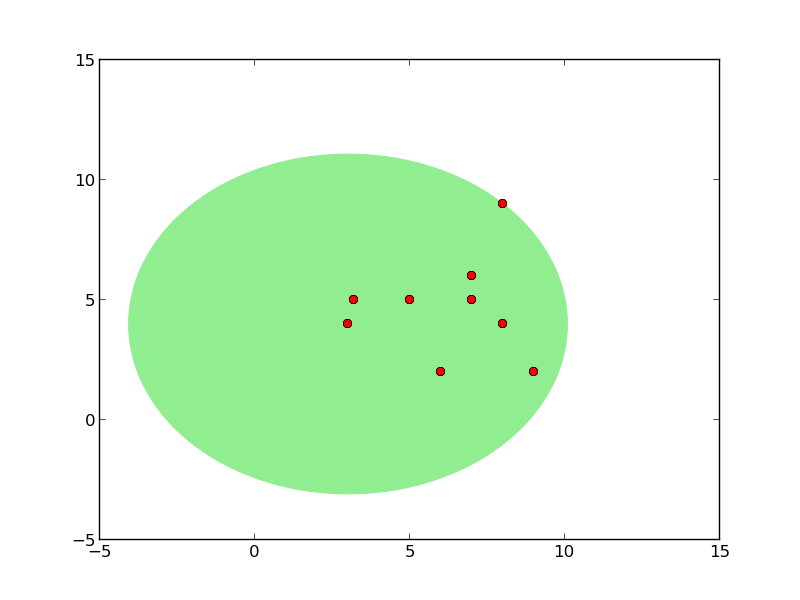
\includegraphics[height=7cm]{pics/knn0.png}

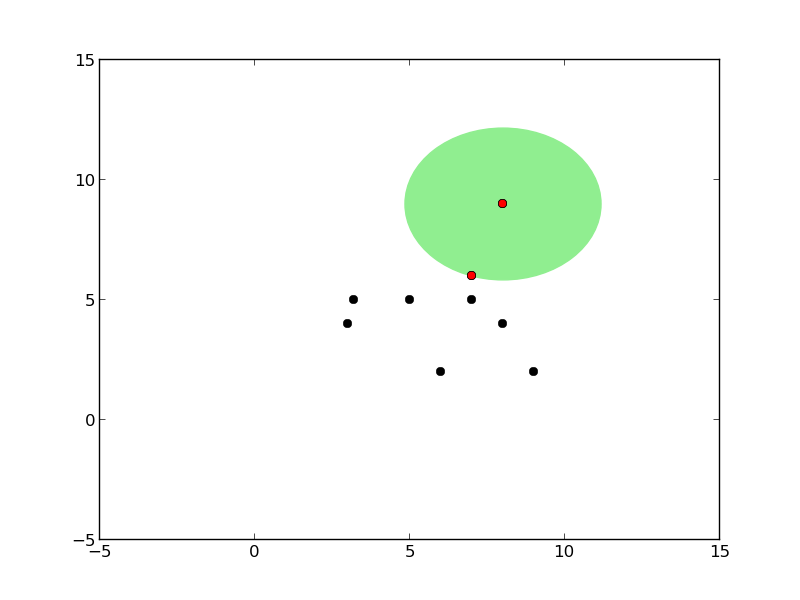
\includegraphics[height=7cm]{pics/knn1.png}

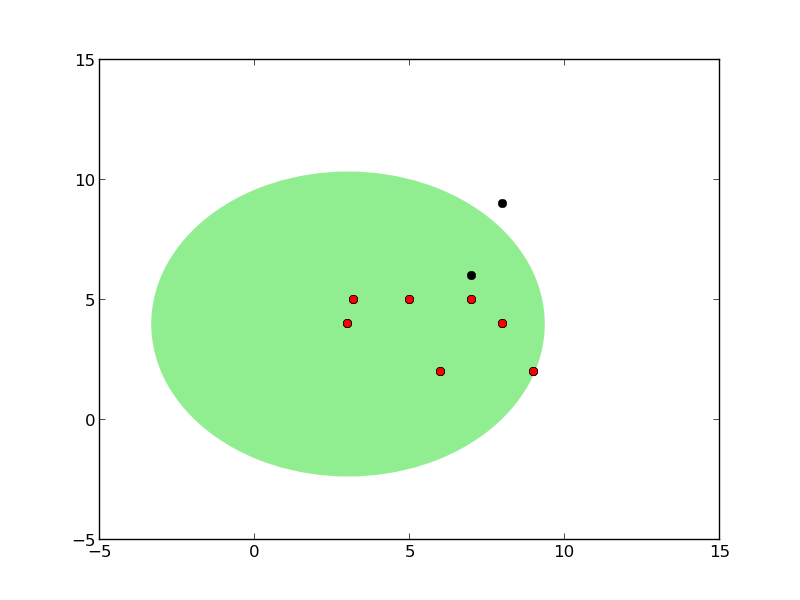
\includegraphics[height=7cm]{pics/knn2.png}

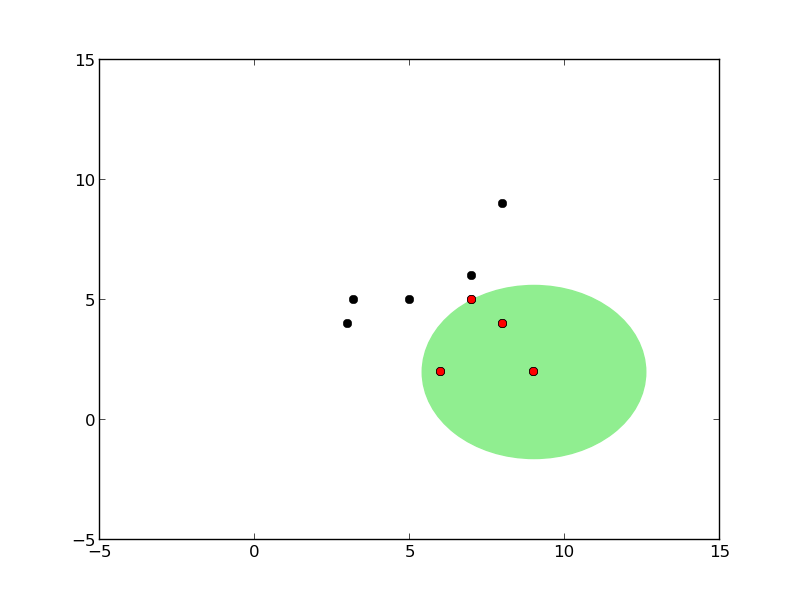
\includegraphics[height=7cm]{pics/knn3.png}

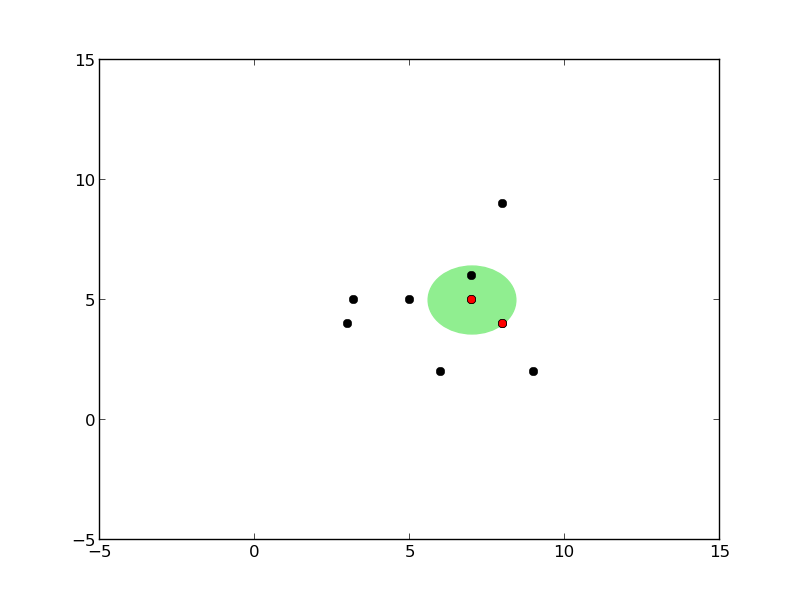
\includegraphics[height=7cm]{pics/knn4.png}

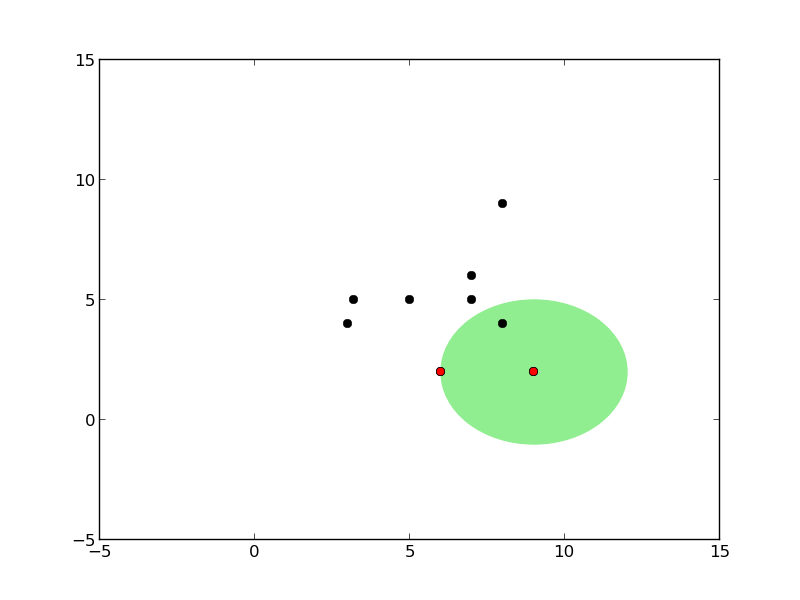
\includegraphics[height=7cm]{pics/knn5.png}

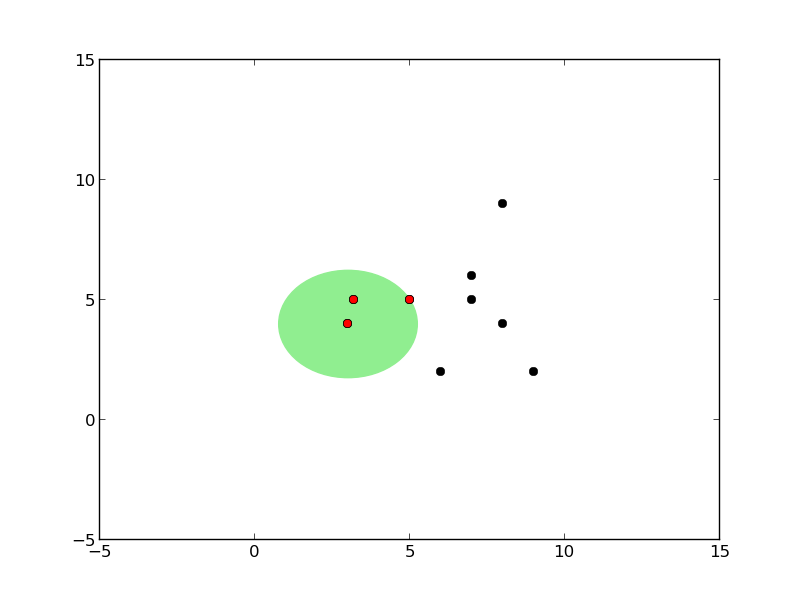
\includegraphics[height=7cm]{pics/knn6.png}

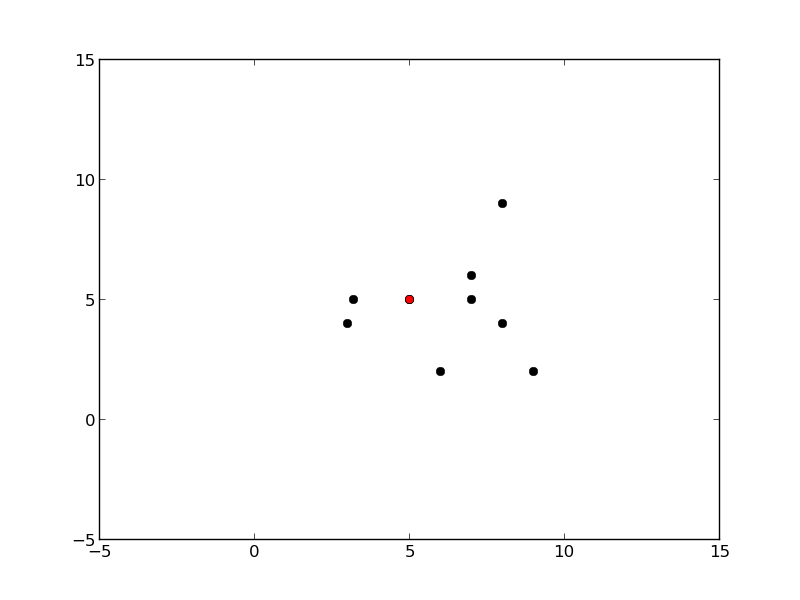
\includegraphics[height=7cm]{pics/knn7.png}

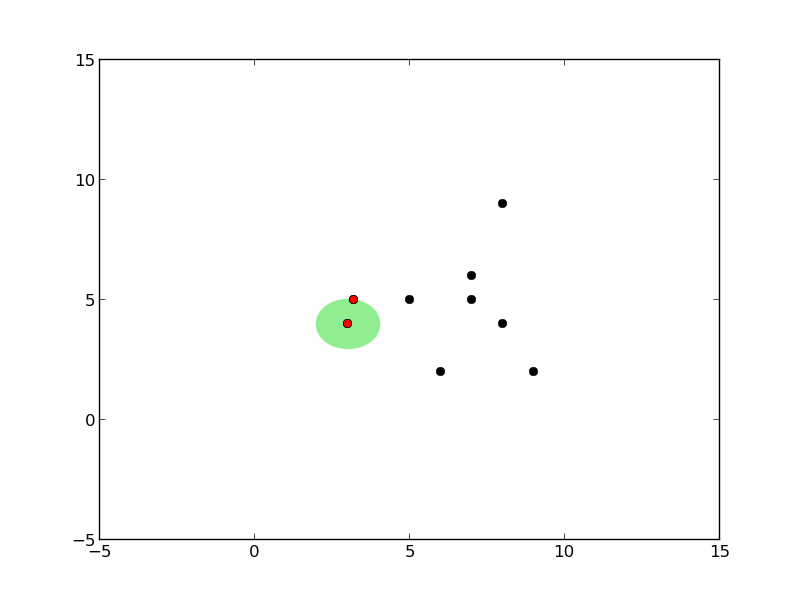
\includegraphics[height=7cm]{pics/knn8.png}



Kaynaklar

[1] Liu, Moore, Gray, {\em New Algorithms for Efficient High Dimensional
Non-parametric Classification}

\end{document}
